\begin{maintask}{1-A}
  \subsection*{課題内容}
  IPv4・IPv6の相手にICMP echo requestを送り，応答の有無を確認した．

  \subsection*{実験方法}
  \begin{enumerate}
    \item 1つ目のターミナルでキャプチャを開始
      \begin{minted}{zsh}
        (IPv4) tcpdump -i eth0 -s 0 -w ping4.pcap
        (IPv6) tcpdump -i eth1 -s 0 -w ping6.pcap
      \end{minted}

    \item キャプチャ中に，別のターミナルでping, ping6を実行
      \begin{minted}{zsh}
        (IPv4) ping -c 5 172.27.0.1
        (IPv6) ping6 -c 5 www.docomo.ne.jp
      \end{minted}
    
    \item pingの終了後，キャプチャ側でCtrl-Cを押し，pcapをダウンロードしてWiresharkで開く
  \end{enumerate}
  
  \subsection*{結果}
  IPv4・IPv6のtcpdumpの実行結果と，ping・ping6の実行結果をそれぞれ
  出力\ref{out:tcpdump_v4}，
  出力\ref{out:tcpdump_v6}，
  出力\ref{out:ping_v4}，
  出力\ref{out:ping_v6}
  に示した．

  \begin{termout}[H]
    \caption{tcpdump(IPv4) の実行結果}\label{out:tcpdump_v4}
    \begin{minted}{zsh}
      guest@host82:~$ tcpdump -i eth0 -s 0 -w ping4.pcap                                                                        
      tcpdump: listening on eth0, link-type EN10MB (Ethernet), capture size 262144 bytes
      ^C14 packets captured
      14 packets received by filter
      0 packets dropped by kernel
     \end{minted}
  \end{termout} 

  \begin{termout}[H]
    \caption{tcpdump(IPv6) の実行結果}\label{out:tcpdump_v6}
    \begin{minted}{zsh}
      guest@host82:~$ tcpdump -i eth1 -s 0 -w ping6.pcap
      tcpdump: listening on eth1, link-type EN10MB (Ethernet), capture size 262144 bytes
      ^C132 packets captured
      146 packets received by filter
      0 packets dropped by kernel
    \end{minted}
  \end{termout}
  
  \begin{termout}[H]
    \caption{ping(IPv4) の実行結果}\label{out:ping_v4}
    \begin{minted}{zsh}
      guest@host82:~$ ping -c 5 172.27.0.1                                                                                      
      PING 172.27.0.1 (172.27.0.1) 56(84) バイトのデータ                                                                               
      64 バイト応答 送信元 172.27.0.1: icmp_seq=1 ttl=64 時間=0.029ミリ秒                                                                    
      64 バイト応答 送信元 172.27.0.1: icmp_seq=2 ttl=64 時間=0.024ミリ秒                                                                    
      64 バイト応答 送信元 172.27.0.1: icmp_seq=3 ttl=64 時間=0.050ミリ秒                                                                    
      64 バイト応答 送信元 172.27.0.1: icmp_seq=4 ttl=64 時間=0.020ミリ秒                                                                    
      64 バイト応答 送信元 172.27.0.1: icmp_seq=5 ttl=64 時間=0.026ミリ秒                                                                    
                                                                                                                                
      --- 172.27.0.1 ping 統計 ---                                                                                                
      送信パケット数 5, 受信パケット数 5, パケット損失 0%, 時間 4097ミリ秒                                                                               
      rtt 最小/平均/最大/mdev = 0.020/0.029/0.050/0.010ミリ秒       
    \end{minted}
  \end{termout}

  \begin{termout}[H]
    \caption{ping6(IPv6) の実行結果}\label{out:ping_v6}
    \begin{minted}{zsh}
      guest@host82:~$ ping6 -c 5 www.docomo.ne.jp                                                                               
      PING www.docomo.ne.jp(2600:9000:2772:3600:7:a2b3:f240:93a1 (2600:9000:2772:3600:7:a2b3:f240:93a1)) 56 データ長(byte)          
      ^C                                                                                                                        
      --- www.docomo.ne.jp ping 統計 ---                                                                                          
      送信パケット数 5, 受信パケット数 0, パケット損失 100%, 時間 4100ミリ秒       
    \end{minted}
  \end{termout}

  \begin{figure}[h]
    \centering
    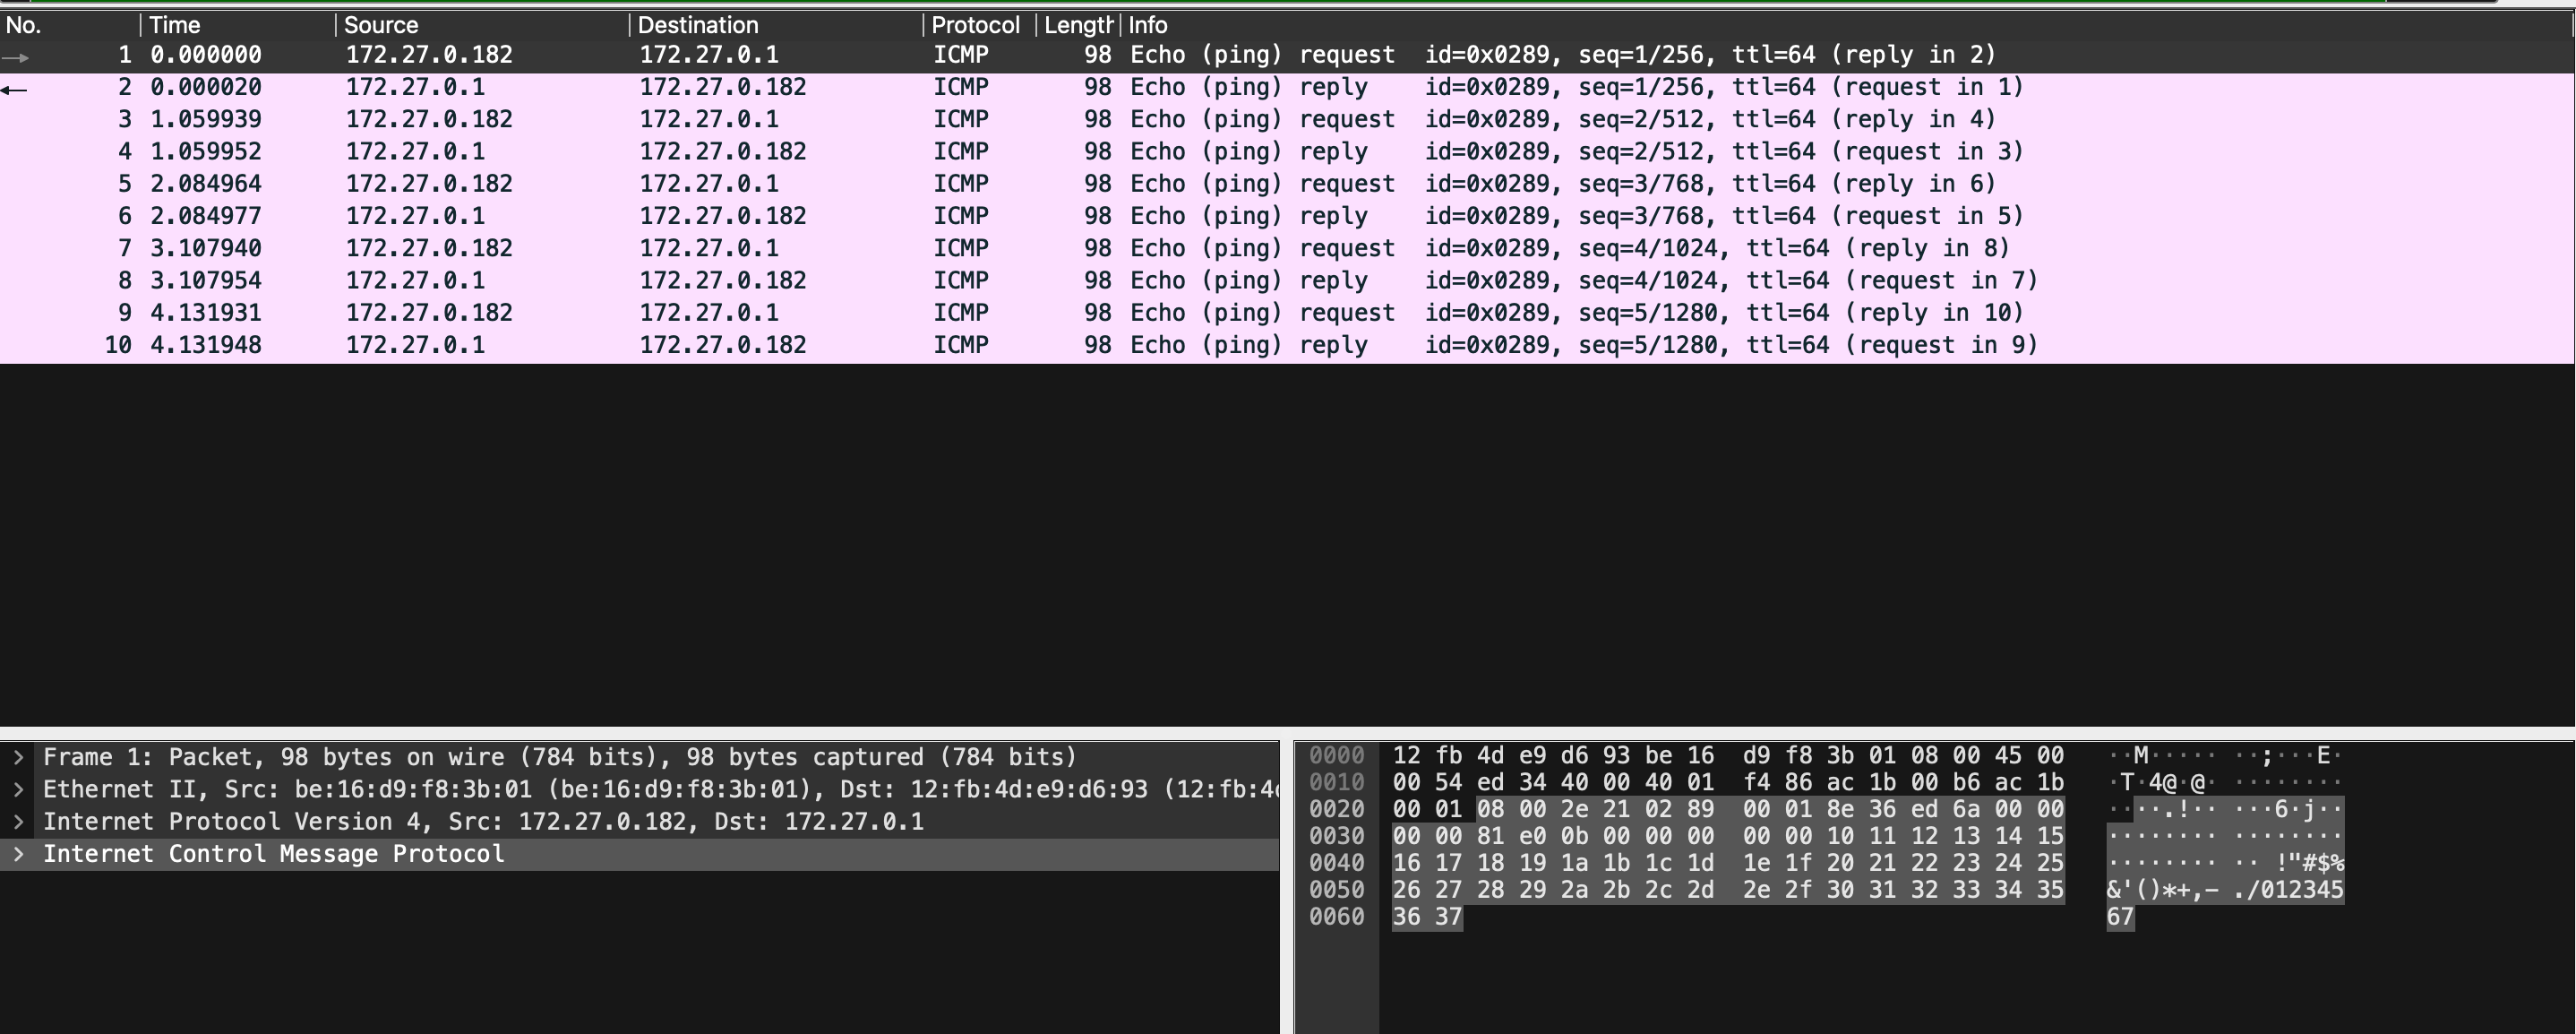
\includegraphics[width=0.98\columnwidth]{fig/wireshark_ipv4.png}
    \caption{IPv4のpingをWiresharkで読み取った結果}
    \label{fig:ws_v4}
  \end{figure}

  \begin{figure}[h]
    \centering
    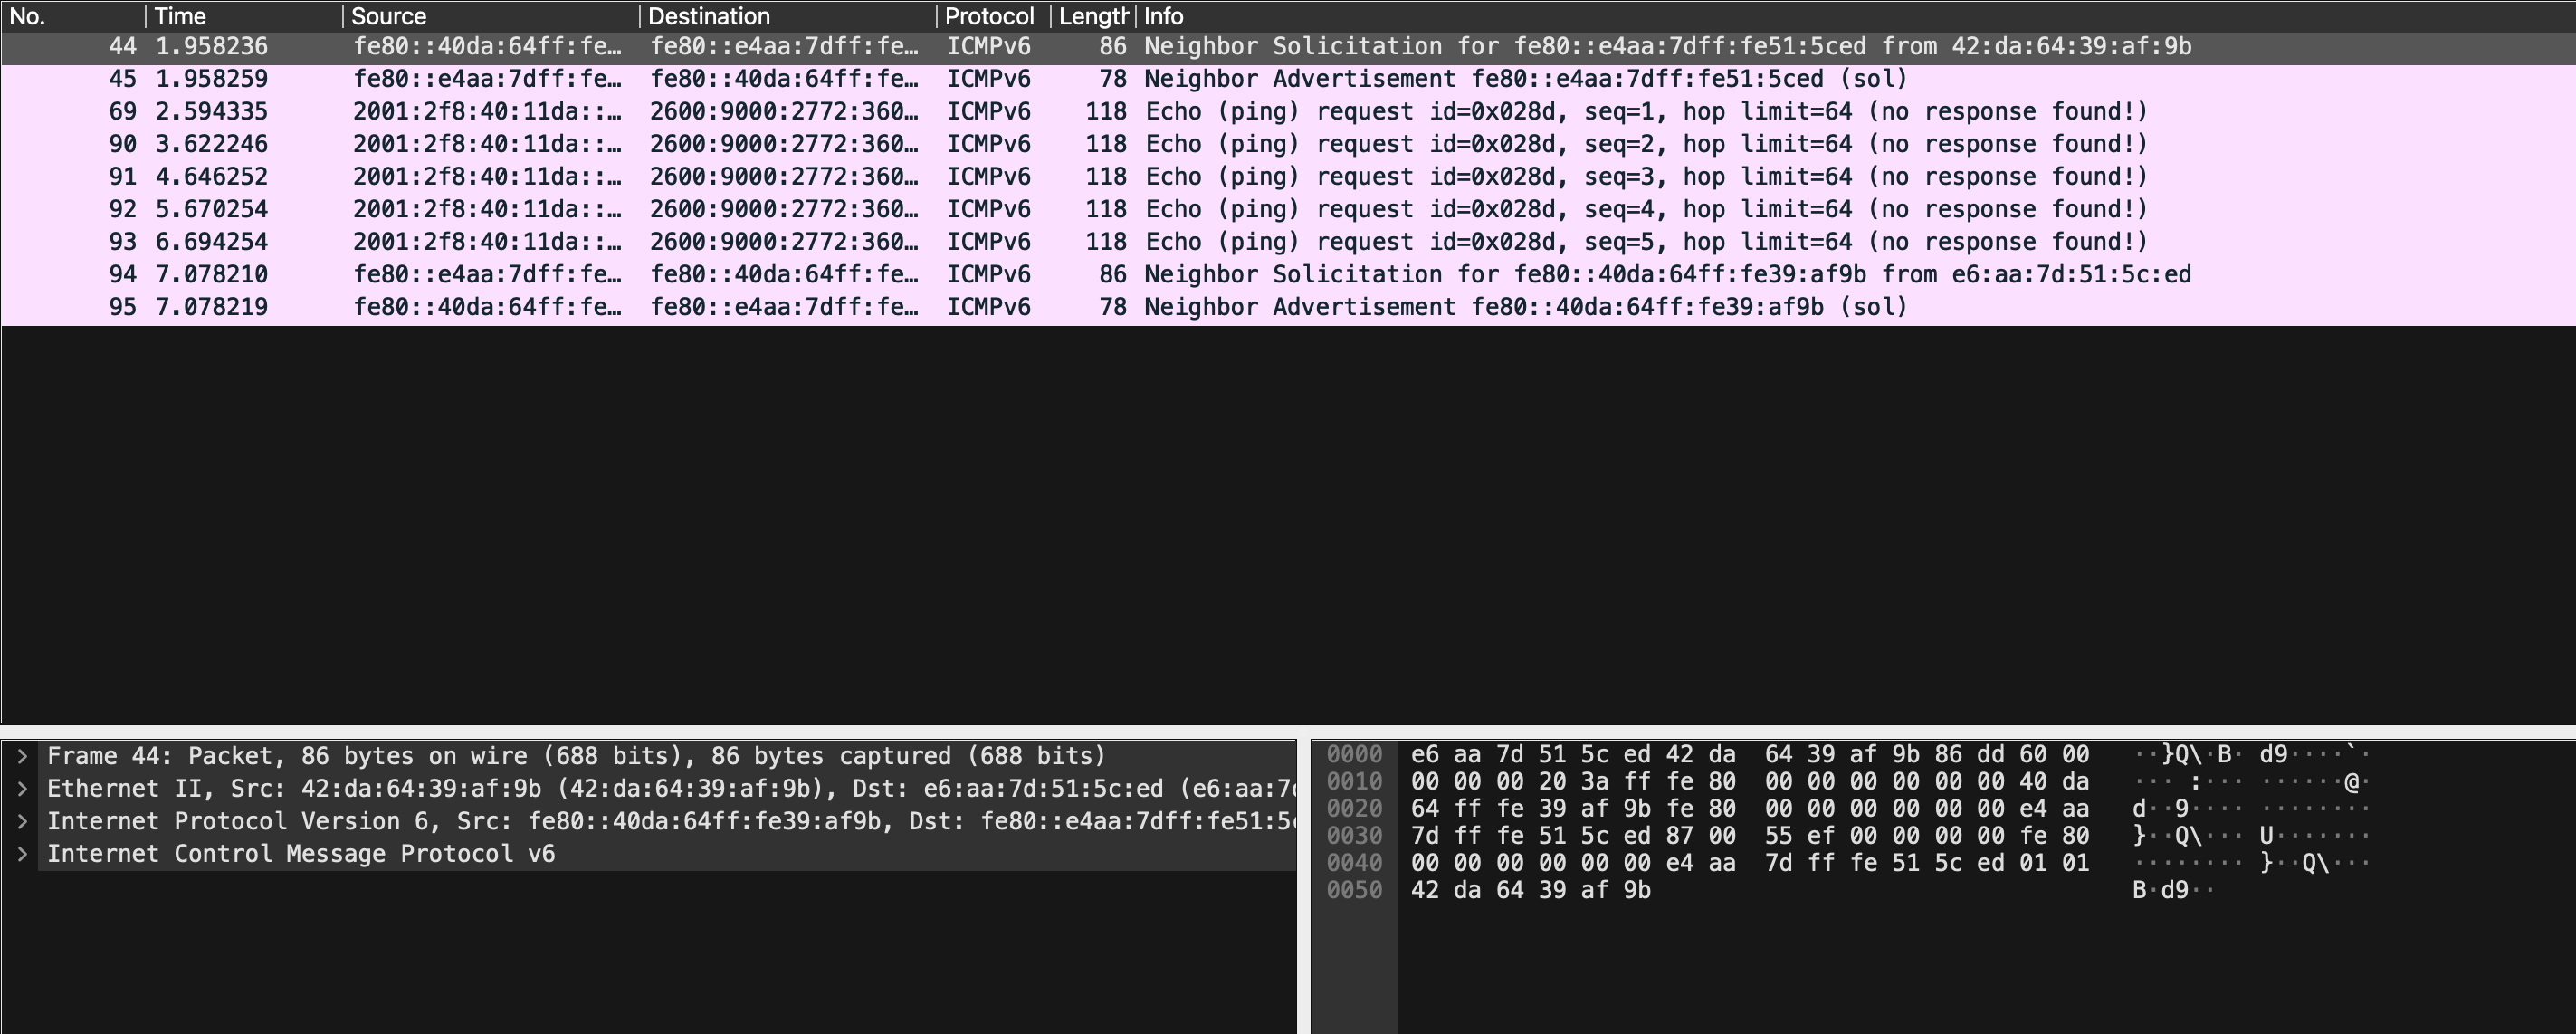
\includegraphics[width=0.98\columnwidth]{fig/wireshark_ipv6.png}
    \caption{IPv6のpingをWiresharkで読み取った結果}
    \label{fig:ws_v6}
  \end{figure}

  IPv4では，送信元172.27.0.182から172.27.0.1に向けてICMP echo requestが5回送信され，それぞれに対するecho replyが確認できた．pingの結果も5パケット送信，5パケット受信であり，パケット損失はなかった．平均往復時間は0.029ミリ秒であった．図\ref{fig:ws_v4}でも，requestとreplyが交互に並んでいることが確認できる．

  IPv6ではwww.docomo.ne.jpの名前解決はでき，2600:9000:2772:3600:7:a2b3:f240:93a1宛てのecho requestが5回送信されたが，echo replyは確認できなかった．pingの結果は5パケット送信，受信0であり，図\ref{fig:ws_v6}にもrequestのみが記録されていた．学外とのICMP通信がネットワーク上で制限されている可能性があるため，この結果だけから通信相手の停止とは判断できない．

\end{maintask}
